%\vspace{-2pt}
\section{{\xblock}: Try-Catch Necessity Checker}
\label{xblock:sec}

\begin{figure}[t]
 	\centering
 	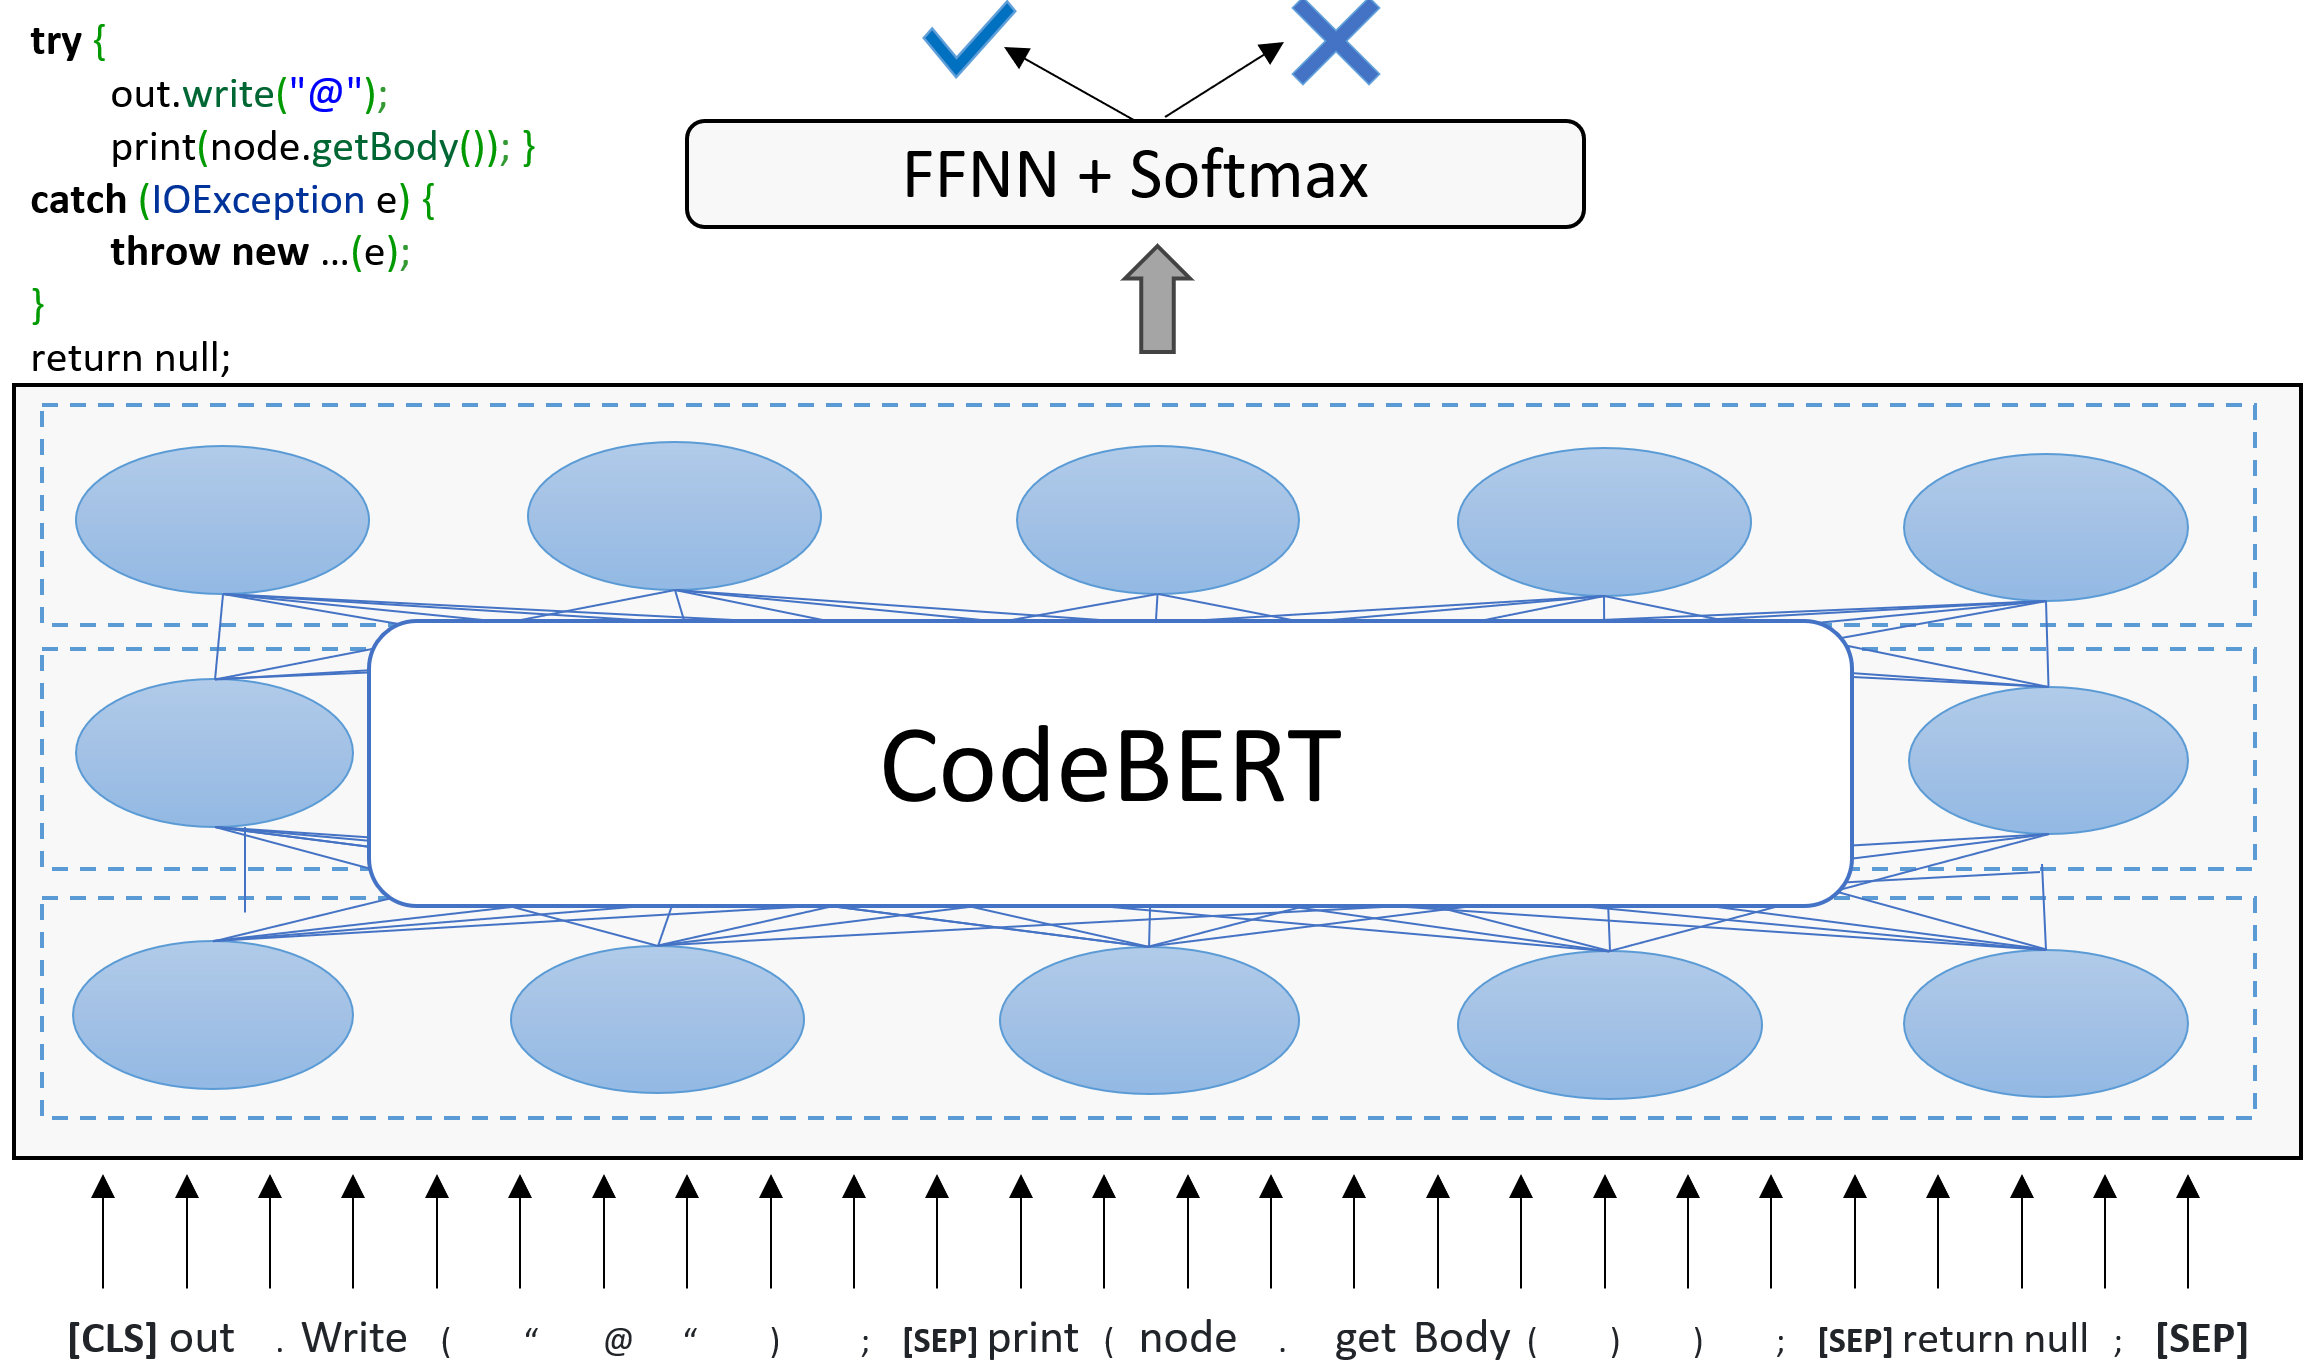
\includegraphics[width=3.4in]{xblock-3.png}
        \vspace{-20pt}
 	\caption{\code{Try-catch} Necessity Checker ({\xblock})}
 	\label{fig:xblock}	
\end{figure}

Given an input code snippet, we first split it into the
statements. Each statement is then tokenized into sub-tokens using the
CodeBERT tokenizer. We use a special separator token \texttt{[SEP]} to
concatenate the tokenized statements, and add a \texttt{[CLS]} token
at the beginning. As in CodeBERT, we take the \texttt{[CLS]} token to
be the representation of the entire code snippet.

We fine-tune a CodeBERT(MLM) for this problem.  Given the good
performance of CodeBERT on many code-related downstream tasks
(https://github.com/microsoft/CodeXGLUE), we expect it to be able to
learn the correlation between important code tokens that would signal
the need of exception handling. Importantly, by providing the code
snippet, we expect to leverage the code context in which the API
elements are used with regard to one another. For example, in
Figure~\ref{overview}, CodeBERT is expected to learn that the APIs
\code{newBufferedReader} of the class \code{Files} and \code{readLine}
of the class \code{BufferedReader} are used often together in API
usages and they require \code{IOException}. For the input incomplete
code snippet, CodeBERT is expected to learn such relations/connections
to avoid name ambiguity and to connect them with the exception types.


During training, as we use exactly one CodeBERT, all three modules
(Sections~\ref{sec:xstate} and~\ref{sec:xtype}) contribute
to the signal for updating the CodeBERT parameters. In {\xblock}, we
feed the vector representation of the \texttt{[CLS]} token to a linear
layer (Feed-forward neural network - FFNN) and use a softmax function
to learn the decision as to whether the input code needs to handle any
exceptions.

% \begin{figure}[t]
% 	\centering
% 	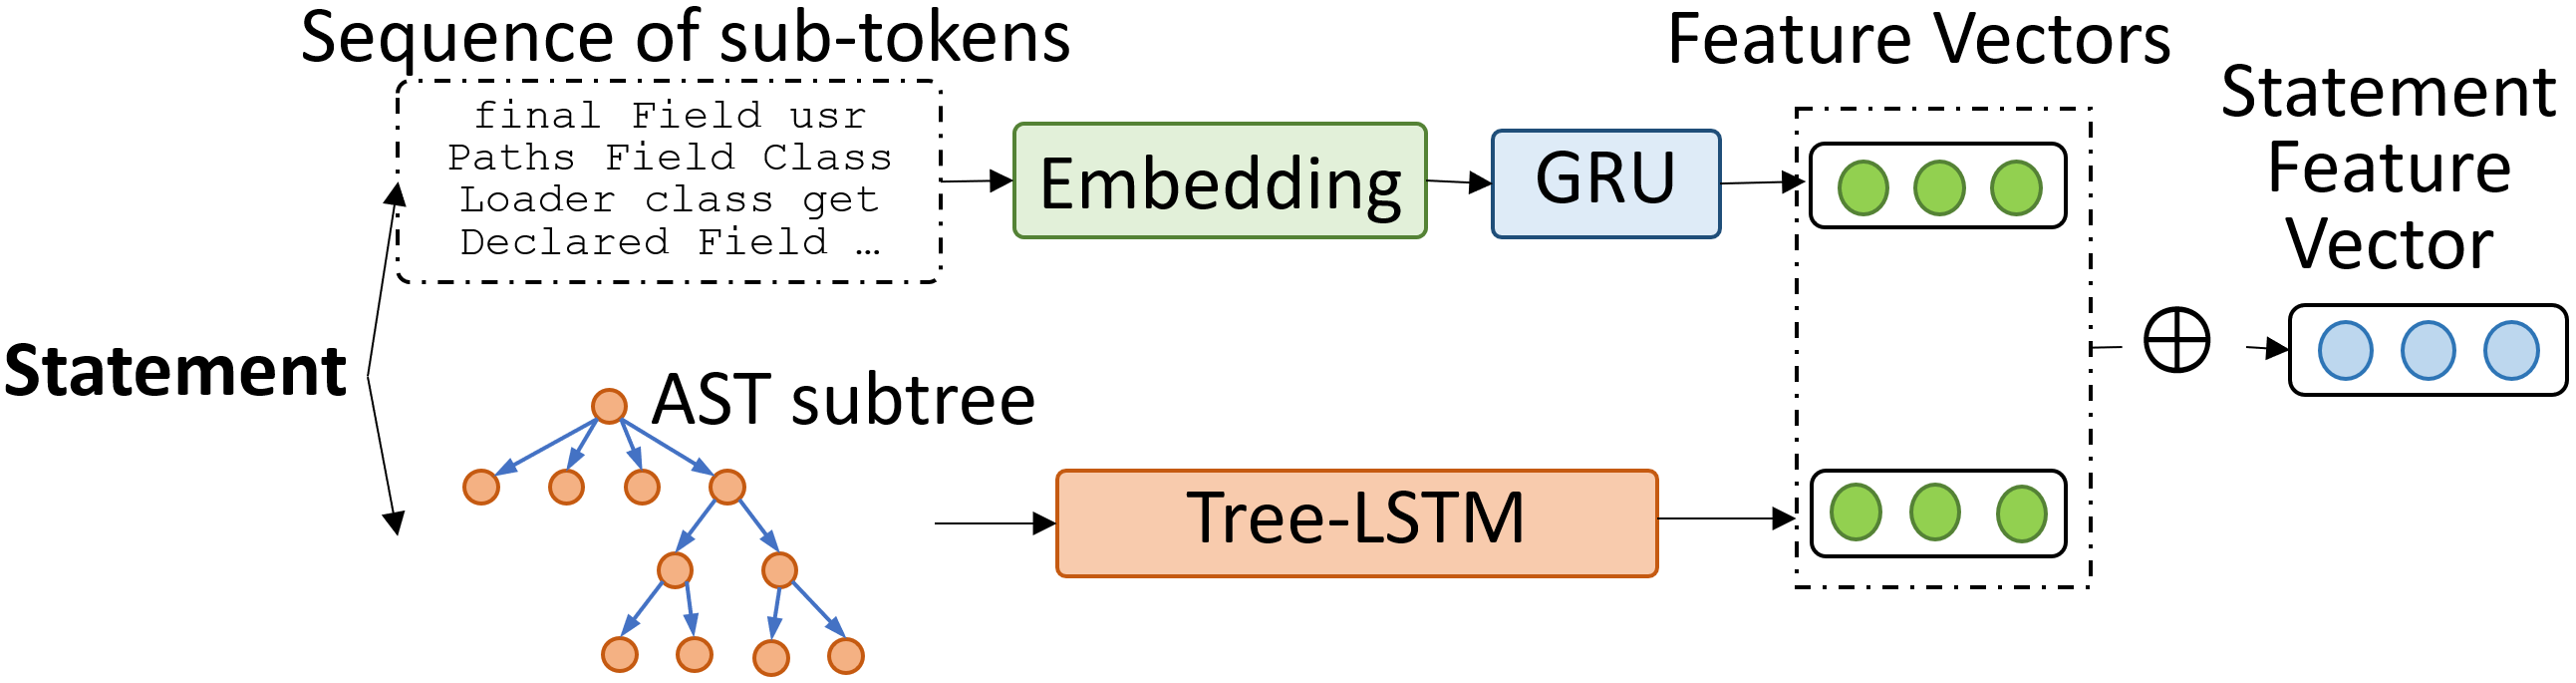
\includegraphics[width=3.2in]{features-2.png}
%         \vspace{-0.08in}
% 	\caption{Code Representation Learning for Statement}
% %        \vspace{-0.05in}
% 	\label{fig:feature}	
% \end{figure}

% %Tien
% %This section describes our graph-based {\xblock} model.

% We first explain how {\xblock} builds the context-aware representation
% learning for the given code, and uses such learned vectors to decide
% if the presence of \code{try-catch} block is needed using
% R-GCN~\cite{rgcn}.

% \subsection{Code Representation Learning}
% \label{replearn:sec}

% Let us explain how we build the vectors for code features
% (Figure~\ref{fig:feature}). We aim to capture the lexical and
% structural features for a statement, while PDG captures the program
% dependencies among statements.

% \vspace{-1pt}
% \subsubsection{Sequence of Sub-tokens of a Statement}

% At the lexical level, a statement is represented via a sequence of the
% sub-tokens. The sub-token granularity has been shown to have higher
% regularity than the tokens~\cite{icse20-methodname}. Each statement is
% tokenized using CamelCase or Hungarian convention. Then, only
% variables, methods, fields, and class' names are kept. The sub-tokens
% with one character are removed to avoid noises. In
% Figure~\ref{fig:example1} at line 2, we collect the sequence of
% sub-tokens as follows: \code{final}, \code{Field}, \code{usr},
% \code{Paths}, etc. We use a word embedding technique~\cite{glove2014}
% to build the vectors for the sub-tokens, together with Gate Recurrent
% Unit (GRU)~\cite{chung2014empirical} to build the feature vector for
% the sequence of sub-tokens for a statement (Figure~\ref{fig:feature}).


% \vspace{-1pt}
% \subsubsection{Code Structure of a Statement}

% At the syntactic level, we aim to capture the code structure via the
% AST. {\tool} parses the code and extracts the AST subtree for the
% given statement, and then feeds it to the Tree-LSTM
% model~\cite{tai2015improved}, which produces a feature vector to
% capture the structure of the statement (Figure~\ref{fig:feature}). If
% the given code is incomplete, we use PPA~\cite{dagenais-oopsla08}, a
% partial program analysis tool to produce the AST for the code in a
% best-effort fashion.


% \subsection{\code{Try-catch} Necessity Checker with R-GCN}
% \label{model:sec}



% Figure~\ref{fig:gcn} illustrates how we use the R-GCN model~\cite{rgcn} to
% detect if a \code{try-catch} block is needed.
% %The rationale is that FA-GCN can deal well with the graphs with sparse
% %features (not all the statements share the same properties), and
% %potentially noisy features in a PDG.
% First, the code is processed by DeepPDA~\cite{icse23}, which is
% capable of parsing any (in)complete code to build the PDG. The
% R-GCN, similar to CNN in image processing, performs a sliding
% window along the nodes in the graph. A window for a node consists of
% its neighboring nodes in the PDG.
% %Similar to CNN using the filter on an image, FA-GCN performs sliding
% %a small window along all the nodes (statements) of the PDG. For
% %example, in Figure~\ref{fig:gcn}, the window marked with A for the
% %node $S27$ consists of itself and the neighboring statements/nodes
% %$S6$, $S22$, $S25$, and $S29$. Another window (marked with B) is for
% %the node $S23$, including itself and the neighboring nodes: $S22$ and
% %$S25$.
% To process a window, the model generates the feature representation
% matrix for the node at the center using the procedure described in
% Figure~\ref{fig:feature}.
% %For example, for the window centered at $S27$, it generates the
% %feature vector $F_{S27}$ for $S27$, using the process explained in
% %Figure~\ref{fig:feature}.
% From the representation vectors for all statements (nodes), the R-GCN
% model will produce the outputs at the output layer. The R-GCN model
% connects all of its outputs to a fully connected layer to transform
% the matrix into a vector $V_C$ to represent the given code
% $C$. {\tool} then performs classification by using a softmax function
% on $V_C$ to decide if a \code{try-catch} block is needed for the
% source code $C$.



